\documentclass[../2.tex]{subfiles}
\begin{document}
    Graphs are used to encode a wide variety of data, from social networks friendships to maps.    
    We can actually consider graphs as the first topological notion introduced in mathematics.
    Their introduction dates back to the XVIII century.
    Euler noticed that in Koningsberg, there was no path that 
    allowed to cross all seven bridges just once. Hence, he started to simplify the problem to approach it in a more mathematical 
    way.
    \begin{figure}[H]
        \begin{minipage}{.5\textwidth}
            \centering
            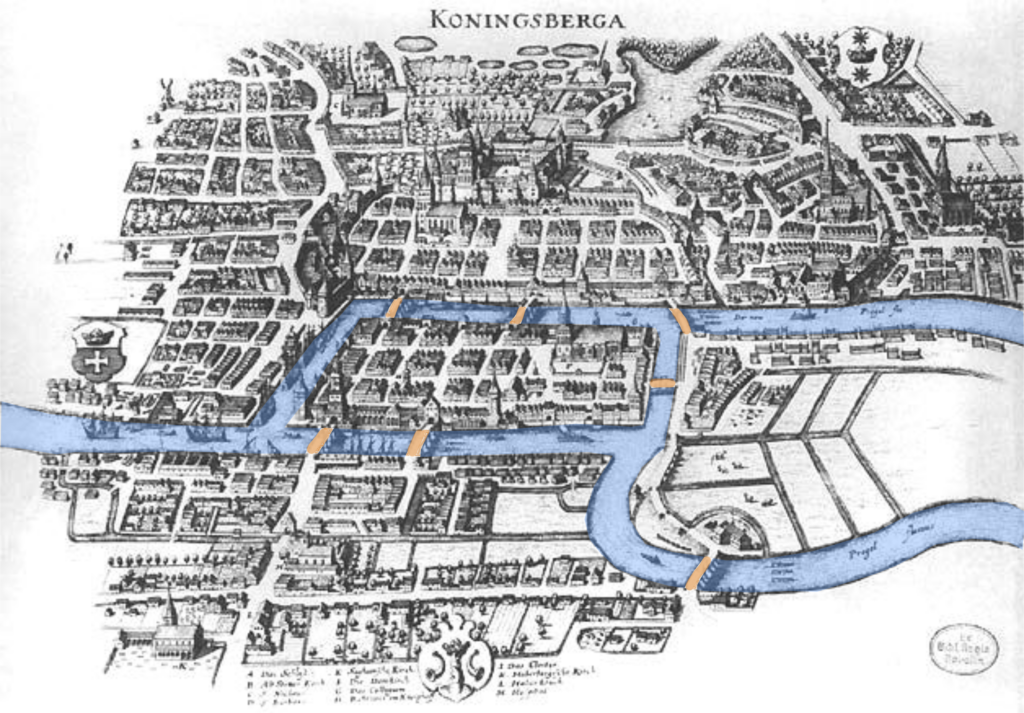
\includegraphics[width=6cm, height=4cm]{sections/2/Bridge}
            \caption{The city of Konigsberg and the\\ seven bridges.}
            \label{fig:2:1}
        \end{minipage}
        \begin{minipage}{.5\textwidth}
            \centering
            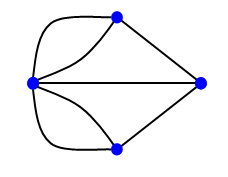
\includegraphics[width=4cm, height=3cm]{sections/2/kgraph}
            \caption{Graph representing Konigsberg's seven bridges.}
            \label{fig:2:2}
        \end{minipage}
    \end{figure}

    This led Euler to formulate an abstract approach to the problem that led to its solution, presented to the St. Petersburg
    Academy in 1735.

    In \autoref{ch:1} we presented abstract simplicial complexes, in this chapter we shall discuss in detail
    $1$-dimensional abstract simplicial complexes and how they are related to graphs. More information
    on graphs can be found in \cite{bondy}.

    \begin{defn}
        An \ii{undirected graph} $\mc{G}$ is an orderd pair $(V(\mc{G}),E(\mc{G}))$, consisting of a set $V(\mc{G})$ of \ii{vertices}
        and a set $E(\mc{G})$, disjoint from $V(\mc{G})$, of \ii{edges}, together with an incidence function
        $\psi_\mc{G}:E(\mc{G}) \to V(\mc{G}) \times V(\mc{G})$ that associates to each edge of $\mc{G}$ an unordered pair of (not necessarily
        distinct) vertices of $\mc{G}$. If $e$ is an edge and $u$ and $v$ are vertices such that $\psi_\mc{G}(e) =
        \{u, v\}$, then $e$ is said to \ii{join} $u$ and $v$, and the vertices $u$ and $v$ are called the \ii{ends}
        of $e$. A graph where the ordering of the ends of an edge is meaningful is said to be a \ii{directed} graph.
    \end{defn}

    Fig. \ref{fig:2:2} represents an undirected graph with four vertices and seven edges.

    \begin{defn}
        Let $\mc{G}$ be an undirected graph, we define the \ii{adjacency matrix} $A$ of $\mc{G}$ as follows,
        $A$ is a $n \times n$ symmetric matrix, where $n$ is the number of vertices, such that
        \[a_{ij} = 
        \begin{cases}
            1 & \text{if there exists an edge joining $i$ with $j$} \\
            0 & \text{otherwise} \\
        \end{cases}. \]        
    \end{defn}

    \begin{rem}
        We can also define the adjacency matrix for directed graphs.
        For a directed graph the adjacency matrix is not symmetric.
    \end{rem}

    \begin{defn}
        A graph is \ii{simple} if it has neither different edges connecting the same pair of verices nor loops, i.e. there is a unique edge joining two different vertices
        and no vertex is joined to itself by an edge. This implies $a_{ii} = 0$ in the adjacency matrix.
    \end{defn}
    
    Much of graph theory is concerned with the study of simple graphs.

    \begin{obs}
        We can view a \ii{simple undirected graph} $\mc{G}$ as $1$-dimensional abstract simplicial complex.
        In fact we can construct a family of sets $\mc{A}$ as in definition \ref{def:1:2:1} in the following way.
        \[ \mc{A} = V(\mc{G}) \cup \{ \{i,j\} \in V(\mc{G}) \times V(\mc{G}) : \exists e \in E(\mc{G}) \quad \psi_\mc{G}(e)=\{i,j\}\}. \]
        It is easy to see that this is an abstract simplicial complex of dimension $1$, one can readily verify the properties in def. \ref{def:1:2:1}.
    \end{obs}

    % In a graph $\mc{G}$ the non trivial chain groups are therefore $C_0(\mc{G})$ and $C_1(\mc{G})$, also called vertex and edge spaces. 
    % The canonical basis of the vertex space is the set of vertexes $\{\ket{i}\}_{i \in I}$, and that of edges which is a subset of $\{\ket{i,j}\}_{(i,j)\in I\times I}$.

    Viewing $\mc{G}$ as a simplicial complex we recall that $C_0$ and $C_1$ are the groups of $0$ and $1$-chains respectively. We denote by $\ch{i}$
    the vertex $i$ as a group element of $C_0$, and we denote $\ch{i,j}$ the edge joining $\ch{i}$ to $\ch{j}$.
    Since $C_1$ is a group, whenever $\ket{i,j} \in C_1$ then also $\ket{j,i} = -\ket{i,j} \in C_1$. 
    
    A canonical basis for $C_0$ is the set of oriented $0$-chains consisting on only one oriented $0$-simplex, 
    similarly for $C_1$.
\end{document}